\documentclass{article}[18pt]
\usepackage[utf8]{inputenc}
\usepackage[margin=0.7in]{geometry}
\usepackage{parselines} 
\usepackage{amsmath}
\usepackage{titlesec}
\usepackage{pgfplots}
\usepackage{graphicx}
\usepackage[english]{babel}
\usepackage{fancyhdr}
\usepackage{circuitikz}
\pgfplotsset{width=10cm,compat=1.9}
\usepackage{relsize}
\titlespacing\section{0pt}{14pt plus 4pt minus 2pt}{0pt plus 2pt minus 2pt}
\newlength\tindent
\setlength{\tindent}{\parindent}
\setlength{\parindent}{0pt}
\renewcommand{\indent}{\hspace*{\tindent}}

\pagestyle{fancy}
\fancyhf{}
\rhead{Sam Robbins 13SE}
\lhead{A Level Physics - Fields}
\rfoot{Page \thepage}


\begin{document}
\begin{center}
\underline{\huge Capacitors}
\end{center}
A capacitor is constructed from two conducting plates separated by an insulator.\\
Charge can flow onto and off the plates but not across the plates.

\section{Charging circuit for a capacitor}
\begin{center}
\begin{circuitikz}[american voltages]
\draw
  (0,0) to [short] (3,0)
  to [battery] (4,0)
  (4,0) to[short] (5,0)
  (4.4,-3) node[spdt](spdt) {}
  (5,0) to[short] (spdt.out 1)
  (spdt.in) to [capacitor] (2,-3)
  (2,-3) to[short] (0,-3)
(0,-3) to[short] (0,0)
(spdt.out 2) to [short] (5,-5) 
(5,-5) to[lamp] (1,-5) 
(1,-5) to[short] (0,-5)
(0,-5) to[short] (0,-3)
  ;
  \end{circuitikz}
  \end{center}
  
When charging the current flows round the top half of the circuit, when discharging the SPDT is changed to the other output and the current flows round the bottom half of the circuit.\\
\\
Capacitors can be used as simple timers in circuits.
\\
\\
The time it takes to charge/discharge depends on:
\begin{itemize}
\item The capacitance of the capacitor \textbf{(C)}
\item The resistance of the charging/discharging circuit \textbf{(R)}
\end{itemize}
\section{Energy stored in a capacitor}
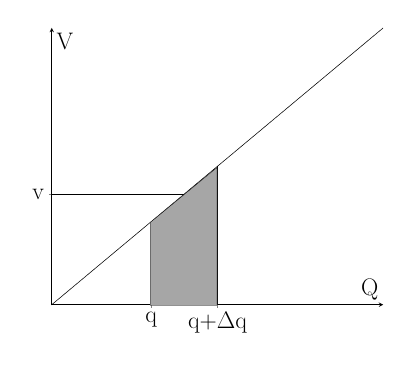
\begin{tikzpicture}[scale=0.5]
\begin{axis}[xmin=0,ymin=-0.01,ylabel=V,xlabel=Q,axis lines=middle,label style={font=\LARGE},
ytick={2},yticklabels=v,
ticklabel style = {font=\LARGE},
xtick={1.5,2.5},xticklabels={q,q+$\Delta$q}
]
\addplot[mark=none]{x};
\addplot [mark=none] coordinates {(1.5,0) (1.5, 1.5)};
\addplot [mark=none] coordinates {(2.5,0) (2.5, 2.5)};
\addplot[mark=none,domain=0:2]{2};
\end{axis}
\filldraw[black, ultra thin,fill=gray!70] (2.5,0) -- (4.2,0) -- (4.2,3.5) -- (2.5,2.1) -- cycle;
\end{tikzpicture}\\
Area under graph=work done\\
V is the average P.D. as charge increases from q to q+$\Delta$q\\
$\Delta \text{w=v}\Delta \text{q}$\\
\\
$Q=\frac{1}{2}QV=E$  \textbf{(Work done=energy stored)}\\
\\
How to answer the exam question: Show that the energy stored by a capacitor is given by $E=\frac{1}{2}QV$
\begin{enumerate}
\item Sketch a graph of Q against V and describe what it shows
\item Describe that electrical energy is the product of charge and voltage
\item State QV is represented by the area under the line
\item The area under the line is a triangle with area =$\frac{1}{2}QV$
\item Therefore $E=\frac{1}{2}QV$
\end{enumerate}
$E=\frac{1}{2}QV$\\
$Q=CV$\\
Therefore:\\
$E=\frac{1}{2}CV^2$\\
$E=\frac{1}{2}\dfrac{Q^2}{C}$\\
\\
The battery supplies energy QV to the circuit but the capacitor only stores $\frac{1}{2}QV$, this means that 50\% of the energy provided by the battery is wasted due to resistance in the circuit.
\section{Charging and discharging a capacitor}
\begin{tikzpicture}[scale=0.5]
\begin{axis}[ticks=none,ylabel=Voltage\textbackslash V,xlabel=Time\textbackslash S,axis lines=middle,
label style={font=\large},xmin=0,xmax=2, 
 x label style={at={(axis description cs:0.5,0)},anchor=north,font=\LARGE},
 y label style={at={(axis description cs:0,.5)},rotate=90,anchor=south,font=\LARGE},
]
\addplot[mark=none,domain=0:2]{1/exp(x)};
\end{axis}
\end{tikzpicture}\\
The smaller the resistor connected to the capacitor, the steeper the initial gradient\\
\\
$\text{p.d.}\propto \text{rate of change of p.d.}$\\
\\
\textbf{Formula for discharge of a capacitor}\\
$\mathlarger{\mathlarger{Q=Q_0e^{-\frac{t}{RC}}}}$\\
\\
Where:\\
Q=Charge at time, t\\
$Q_0$=Initial charge\\
\\
$\mathlarger{\mathlarger{e^{-\frac{t}{RC}}}}$=Multiplication factor between 0 and 1\\
\\
This also works for:\\
\\
$\mathlarger{\mathlarger{V=V_0e^{-\frac{t}{RC}}}}$\\
\textbf{Formula for charging of a capacitor}\\
$\mathlarger{\mathlarger{Q=Q_0(1-e^{-\frac{t}{RC}})}}$\\
\\
\textbf{Rearranging for time}\\
\\
$\mathlarger{\mathlarger{V=V_0e^{-\frac{t}{RC}}}}$\\
\\
$\dfrac{V}{V_0}=e^{-\frac{t}{RC}}$\\
$\ln\Big(\dfrac{V}{V_0}\Big)=-\dfrac{t}{RC}$\\
$t=-RC\ln\Big(\dfrac{V}{V_0}\Big)$\\
$t=RC\ln\Big(\dfrac{V_0}{V}\Big)$\\
\\
\subsection{Proof of the units of the time constant being seconds}
$\tau=RC$\\\\
$\tau=\dfrac{V}{I}\times\dfrac{Q}{V}=\dfrac{Q}{I}$\\
\\
$\dfrac{Q}{I}=t$(unit seconds)
\section{Capacitor Discharge Theory}
RC controls the date of discharge
\subsection{How much time remains after 1 time constant}
$Q=Q_0e^{-\frac{t}{RC}}$\\
\\
$Q=Q_0e^{-\frac{RC}{RC}}$\\
\\
$Q=Q_0e^{-1}$\\
\\
$e^{-1}$ is approximately 37\%, this means that when charge is 37\% of the initial value, 1 time constant will have passed.
\subsection{Alternate way of finding the time constant}
The $x$ intercept of the graph of voltage against time if the initial gradient is continued is the time constant.
\subsection{3rd method of finding the time constant}
The formula $V=V_0e^{-\frac{t}{RC}}$ can be rearranged to $RC=\dfrac{t}{\ln(\frac{v_0}{v})}$.\\
This means that using the initial voltage and the voltage at a point in time, the time constant can be calculated.
\section{Dielectrics}
Capacitance is increased by placing an insulator between the plates of a capacitor.\\
\\
This means that more charge is stored on the capacitor for a given p.d. as:
\begin{itemize}
\item The positive side of the dielectric attracts more electrons from the supply
\item The negative side of the dielectric pushes more electrons towards the supply
\end{itemize}
$$ Q\propto C$$
\section{Relative permittivity}
This is the ration of charge stored with the dielectric compared to the charge stored with no dielectric.\\
$$\epsilon_r=\dfrac{Q}{Q_0}$$
$$\epsilon_r=\dfrac{C}{C_0}$$
$$\epsilon=\epsilon_0\epsilon_r$$
\subsection{Capacitor design}
$C=\dfrac{A\epsilon_0\epsilon_r}{d}$ Therefore $C\propto A \quad C\propto \epsilon_r \quad C\propto \frac{1}{d}$
\end{document}
